\documentclass[tikz]{standalone}

\begin{document}
	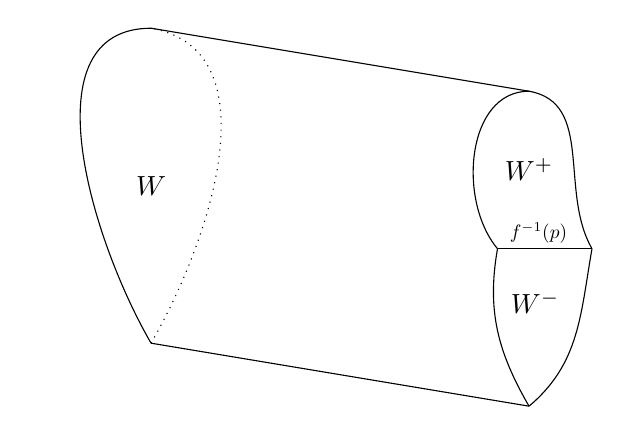
\begin{tikzpicture}[scale=4]
	\coordinate (a)  at (0,1.2);
	\coordinate (b)  at (0,0.2);
	\coordinate (c)  at (1.2,1);
	\coordinate (d1) at (1.1,.5);
	\coordinate (d2) at (1.4,.5);
	\coordinate (e)  at (1.2,0);

	\draw[out=120, in=180]        (b) to (a);
	\draw[out=60, in=-10, dotted] (b) to (a);

	\draw (a) -- (c);
	\draw (b) -- (e);

	\draw[out=180, in=130] (c) to (d1);
	\draw[out=-10, in=120] (c) to (d2);
	\draw[out=-100, in=120] (d1) to (e);
	\draw[out=-100, in=40] (d2) to (e);

	\draw (d1) to (d2);

	\node at (0, .7) {$W$};
	\node at (1.2, .75) {$W^+$};
	\node[scale=.7] at (1.23, .55) {$f^{-1}(p)$};
	\node at (1.22, .33) {$W^-$};
	\end{tikzpicture}
\end{document}